\documentclass{gescons}

\genre {Editorial}
\author{Amanda Vieira}
\authorrole{Editora desta Edição}
\title{20 anos de Publicação Interassistencial: Passado, Presente e~Futuro da Editares}

\begin{document}
    \makeentrevistatitle
    %\maketitle

    %\fullwidthimage{fields}{b}

    \coverart{back/editorial}
    %\coverart{../fundo-generico.png}

    \begin{multicols}{2}

%\begin{center}
%    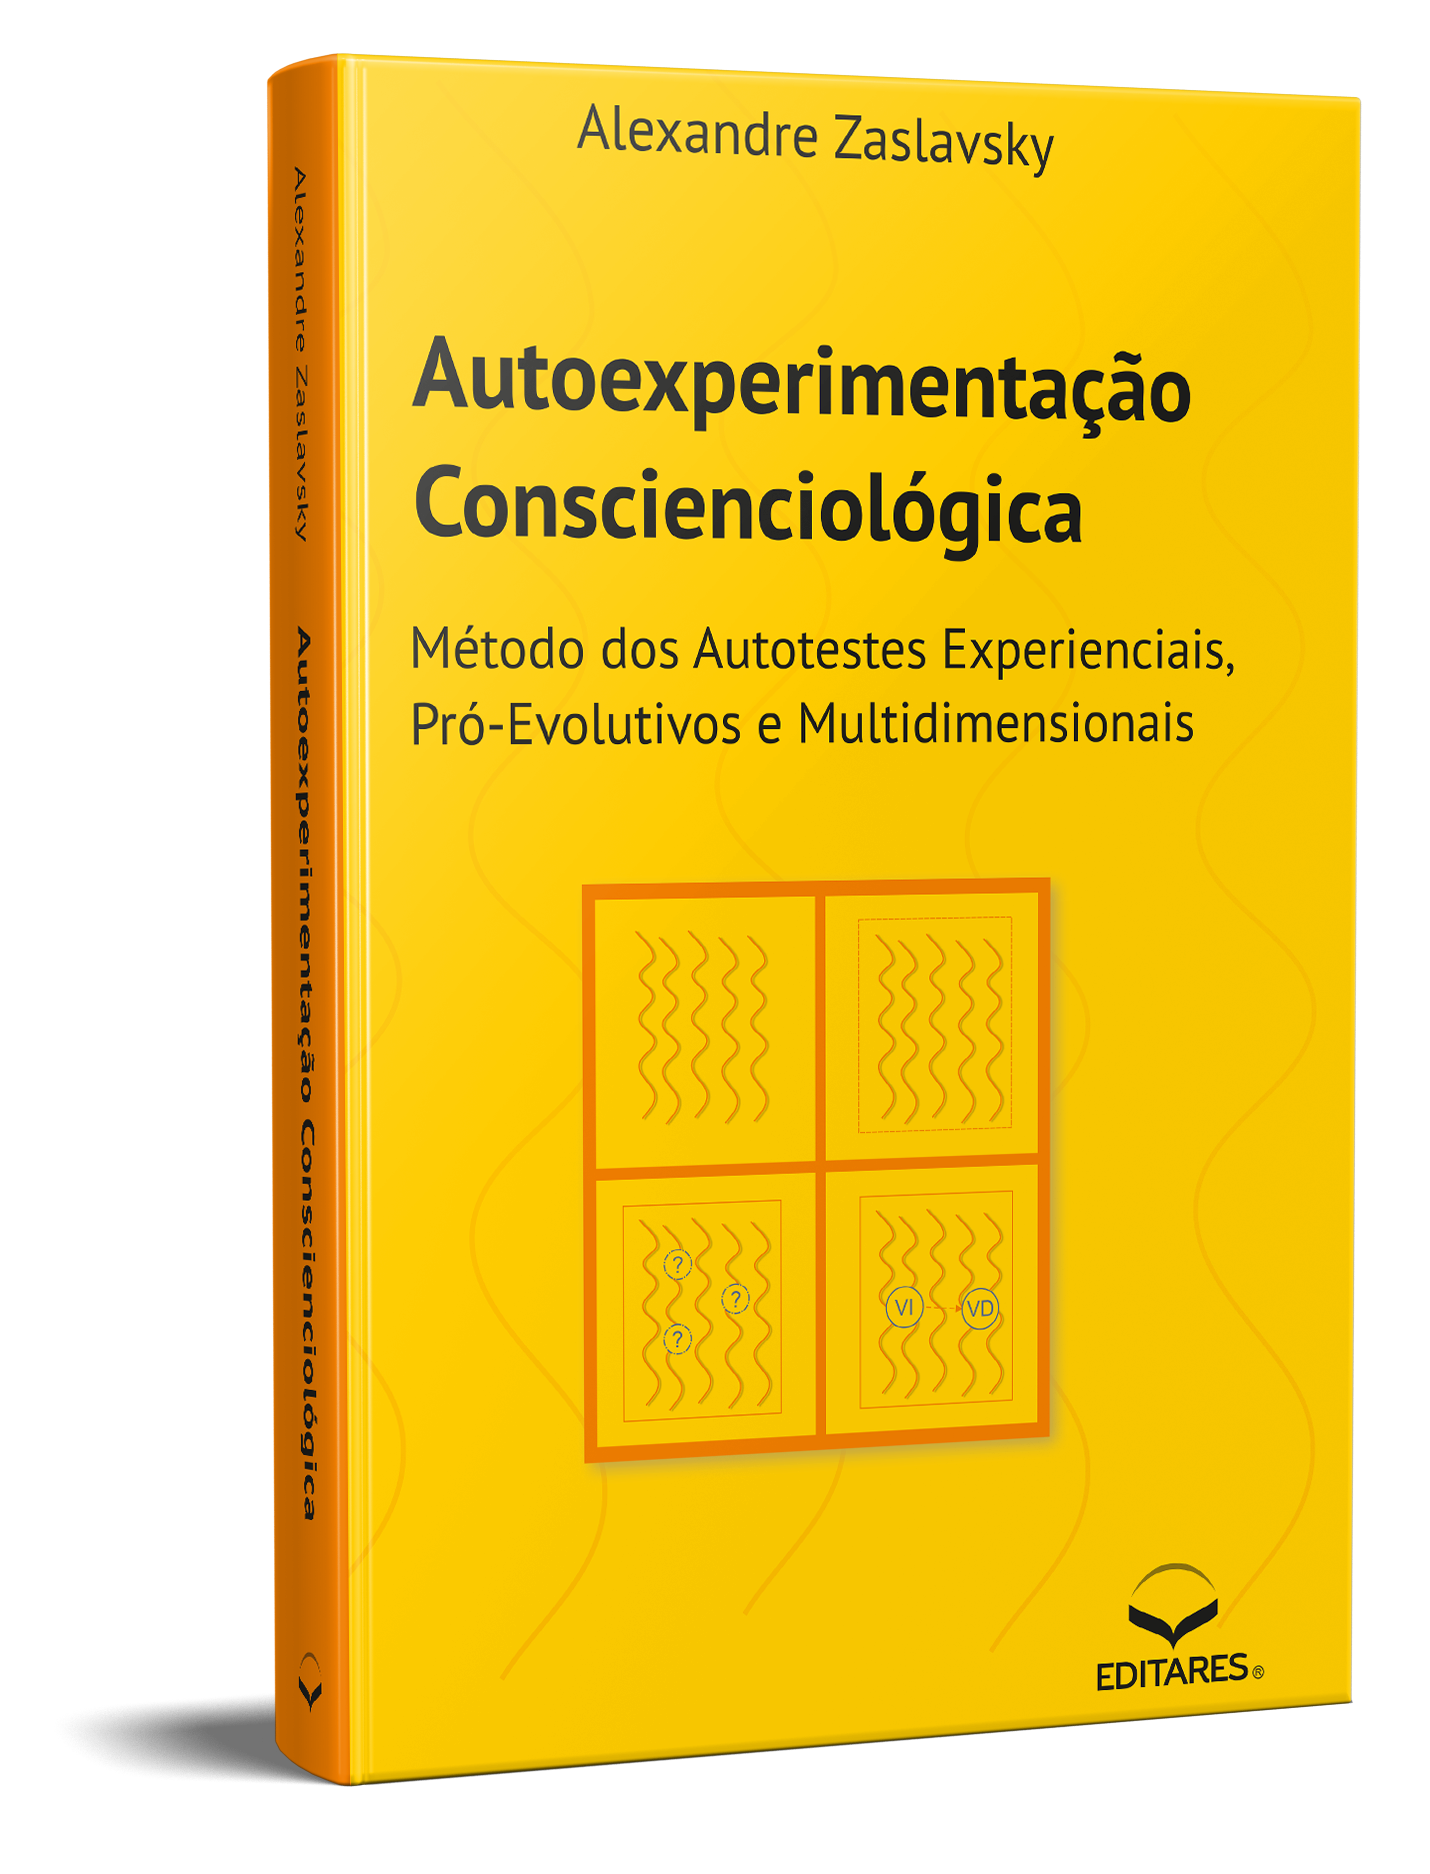
\includegraphics[width=4cm]{articles/entrevista/mockups/Alexandre-Zas.png}
%\end{center}

Em 2024, a~Editares completou 20 anos de dedicação à~publicação técnico-científica de obras conscienciológicas. Duas décadas de trabalho tarístico, construídas por muitas mãos, em que cada autor, revisor, diagramador, conselheiro, voluntário e~leitor fez parte de um mesmo propósito: \textbf{expandir o~esclarecimento e~favorecer a~evolução das consciências por meio da escrita.}

Celebrar essa história significa reconhecer o~valor do esforço coletivo. Desde os primeiros livros publicados até os mais recentes lançamentos, cada obra representa um marco de interassistência, registrando aprendizados, reflexões e~contribuições para o~desenvolvimento da Conscienciologia e~para a~maxiproéxis grupal.

Esta edição da Revista Gescons propõe um olhar integrado sobre a~trajetória da Editares: passado, presente e~futuro se encontram para inspirar novos desafios e~conquistas. É~um convite para pensar no que já realizamos juntos e,~principalmente, no que ainda podemos alcançar coletivamente.

Na primeira seção, apresentamos \textbf{resumo do biênio} com os acontecimentos mais relevantes da Editares entre 2024 e~2025: a~conquista da Certificação Institucional da UNICIN, a~participação no Congraçamento das ICs, a~distribuição internacional de materiais no Japão e~na Europa, as atualizações do fluxo editorial e~os números que refletem nossa produção recente. Um destaque especial vai para a~listagem completa dos voluntários atuais, organizados por equipes de trabalho, valorizando quem faz a~Editares acontecer.

Na segunda seção, trazemos \textbf{atualizações} e~novidades institucionais: a~criação da Escola de Editores, voltada à~formação e~qualificação de novos voluntários; as novas estratégias de \emph{marketing}; e~a~nova revista científica da Editares para expansão da especialidade Editoriologia e~Publicaciologia. 

Na terceira seção, compartilhamos sobre a~reativação da parceria com o~IIPC para ampliar a~venda de livros; apresentamos o~novo acordo firmado com a~Uniescon; e~os grupos de trabalho com a~UNICIN, responsáveis por repensar processos comerciais e~editoriais.

Por fim, na quarta seção apresentamos os \textbf{lançamentos de 2024 e~2025,} com obras que ampliam o~debate técnico e~aprofundam a~pesquisa conscienciológica.

Mais do que celebrar o~passado, esta edição propõe \textbf{um olhar para o~futuro.} Queremos inspirar novos autores, atrair mais voluntários e~consolidar práticas editoriais cada vez mais qualificadas e~pautadas na interassistência. Seguimos firmes no propósito de transformar ideias em livros, livros em esclarecimento e~esclarecimento em evolução.

Agradecemos a~todos os voluntários, autores, leitores e~parceiros que fazem parte desta história. Que os próximos anos sejam ainda mais produtivos, lúcidos e~marcados pela interassistência.

Boa leitura!

%\begin{center}
%    %  trim={<left> <lower> <right> <upper>}
%    \includegraphics[width=8cm,trim={0 200 0 70},clip]{articles/inicial/imagens/Amanda.jpeg}
%\end{center}

%\begin{pullquote}
%``A escrita de uma obra conscienciológica é~uma oportunidade evolutiva inigualável.''
%\end{pullquote}

        
    \end{multicols}

% \begin{figure}[h] % [htbp] are placement options (here, top, bottom, page)
% \centering % Centers the image and caption
% \includegraphics[width=5cm,trim={0 200 0 70},clip]{articles/editorial/imagens/Amanda.jpeg}
% \caption*{Editora desta Edição} % The caption text
% \end{figure}

\end{document}
